\documentclass[UTF8, a4paper, 11pt]{article}
\usepackage{subfigure}
\usepackage[UTF8, scheme=plain]{ctex}
\usepackage{fontspec}
\usepackage{float}
\usepackage{amsmath}
\newtheorem{myDef}{Definition}
\usepackage{graphicx}
\usepackage{geometry}
\usepackage{listings}
\usepackage{xcolor}
\usepackage{caption}
\geometry{scale=0.8}
\linespread{1.5}
\usepackage{hyperref}
\usepackage{color}
\usepackage{fontspec}
\usepackage{enumitem}
\usepackage[linesnumbered,boxed]{algorithm2e}
\usepackage{xeCJK}
\usepackage{indentfirst} 
\graphicspath{{Pics/}} 	% 在于.tex同级的目录下创建名为pic的文件夹,存放图片


\setlength{\parindent}{2em}

\lstset{
    language={sql},
    frame=shadowbox,
    breaklines=true,
    numbers=left,
    backgroundcolor=\color[RGB]{245,245,244},
    rulesepcolor=\color{red!20!green!20!blue!20},
    numberstyle={\color[RGB]{0,192,192}\tiny},
    basicstyle=\footnotesize \fontspec{Source Code Pro}
}
\setenumerate[1]{itemsep=0pt,partopsep=0pt,parsep=\parskip,topsep=0pt}
\setitemize[1]{itemsep=0pt,partopsep=0pt,parsep=\parskip,topsep=0pt}
\setdescription{itemsep=0pt,partopsep=0pt,parsep=\parskip,topsep=0pt}


\title{	
\normalfont \normalsize
\textsc{School of Data and Computer Science, Sun Yat-sen University} \\ [25pt] %textsc small capital letters
\rule{\textwidth}{0.5pt} \\[0.4cm] % Thin top horizontal rule
\huge 功能简介和数据库部分实现\\ % The assignment title
\rule{\textwidth}{2pt} \\[0.5cm] % Thick bottom horizontal rule
\author{18308045 Zhengyang Gu}
\date{\normalsize\today}
}

\begin{document}
\maketitle
\tableofcontents
\newpage
\section{功能简介}
总体来说是图书售卖系统。具体来说,包含以下几个功能:
\begin{enumerate}
    \item 创建管理员用户,管理员用户可以管理数据库。
    \item 创建普通用户。
    \item 如果图书还有余量,则可购买此图书。
    \item 如果用户已经购买过图书,则可评价此图书。
    \item 创建书单其中有标题和描述,所有用户都可以查看,并按照书单买书(好书推荐)。
\end{enumerate}

\section{具体实现}
\subsection{模式设计}
\subsubsection{ER图}
\begin{figure}[H]
    \centering
    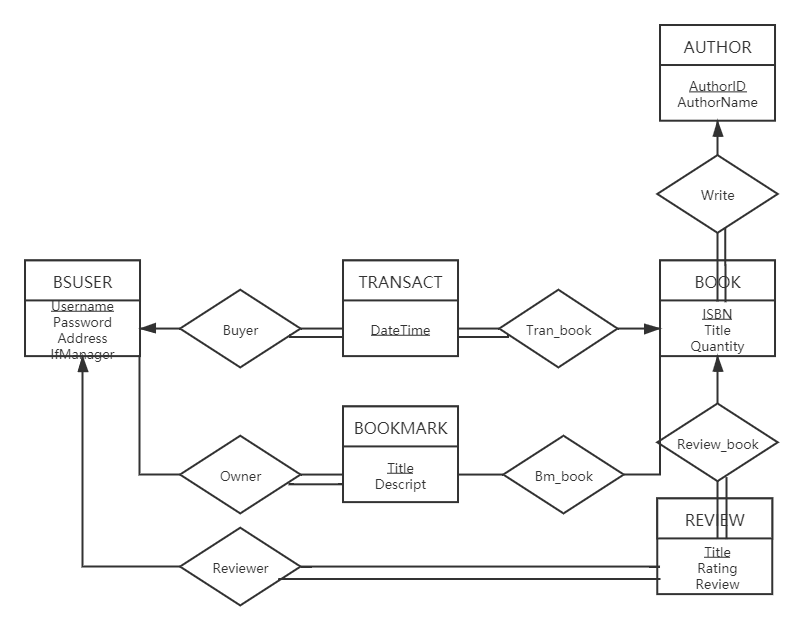
\includegraphics[width = 0.8 \textwidth]{ER.png}
\end{figure}
\subsubsection{转化为模式}
一对多的,让多的实体包含一的实体的主码;多对多的,增加一个表包含两个实体。另外值得注意的是对书的数目即quantity设了一个约束大于等于0。
\begin{lstlisting}
CREATE TABLE BSUSER
(
    Username VARCHAR(15) NOT NULL,
    Password VARCHAR(15) NOT NULL,
    Address VARCHAR(20) NOT NULL,
    IfManager INT,
    PRIMARY KEY(Username)
);

CREATE TABLE AUTHOR
(
    AuthorID VARCHAR(15) NOT NULL,
    AuthorName VARCHAR(15) NOT NULL,
    PRIMARY KEY(AuthorID)
);

CREATE TABLE BOOK
(
    ISBN CHAR(14) NOT NULL,
    Title VARCHAR(50) NOT NULL,
    AuthorID VARCHAR(15) NOT NULL,
    Quantity INT NOT NULL,
    CHECK (Quantity >= 0),
    PRIMARY KEY(ISBN),
    FOREIGN KEY(AuthorID) references AUTHOR(AuthorID)
);

CREATE TABLE REVIEW
(
    Title VARCHAR(15),
    Reviewer VARCHAR(15) NOT NULL,
    BookID CHAR(14) NOT NULL,
    Rating INT NOT NULL,
    Review TEXT,
    CHECK (Rating >= 1 OR Rating <= 5),
    PRIMARY KEY(Title),
    FOREIGN KEY(Reviewer) references BSUSER(Username),
    FOREIGN KEY(BookID) references BOOK(ISBN)
);

CREATE TABLE TRANSACT
(
    DateTime CHAR(23) NOT NULL,
    Buyer VARCHAR(15) NOT NULL,
    BookID CHAR(14) NOT NULL,
    PRIMARY KEY(DateTime),
    FOREIGN KEY(Buyer) references BSUSER(Username),
    FOREIGN KEY(BookID) references BOOK(ISBN)
);

create table BOOKMARK
(
    Title VARCHAR(15),
    Descript TEXT,
    primary key(Title)
)

create table BOOKMARK_BOOK
(
    Title VARCHAR(15),
    Owner VARCHAR(15),
    BookID CHAR(14),
    Owned Bit,
    primary key(Title, BookID, Owned),
    foreign key(Owner) references BSUSER(Username),
    foreign key(BookID) references BOOK(ISBN)
)
\end{lstlisting}
\subsection{触发器}
\subsubsection{评论}
要求评论书前,需要已经购买过此书:
\begin{lstlisting}
create trigger t_reivew on REVIEW for insert as
if (select count(*)
    from TRANSACT t, inserted i
    where t.Buyer=i.Reviewer and t.BookID=i.BookID)=0
begin
rollback TRANSACTION
end
\end{lstlisting}
测试恶意评论结果如下:
\begin{figure}[H]
    \subfigure{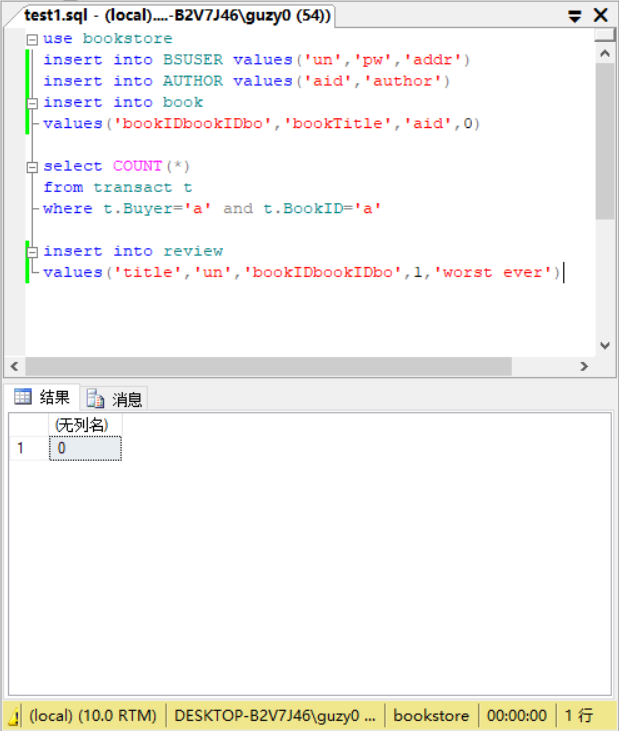
\includegraphics[width = 0.5 \textwidth]{test1re.png}}
    \subfigure{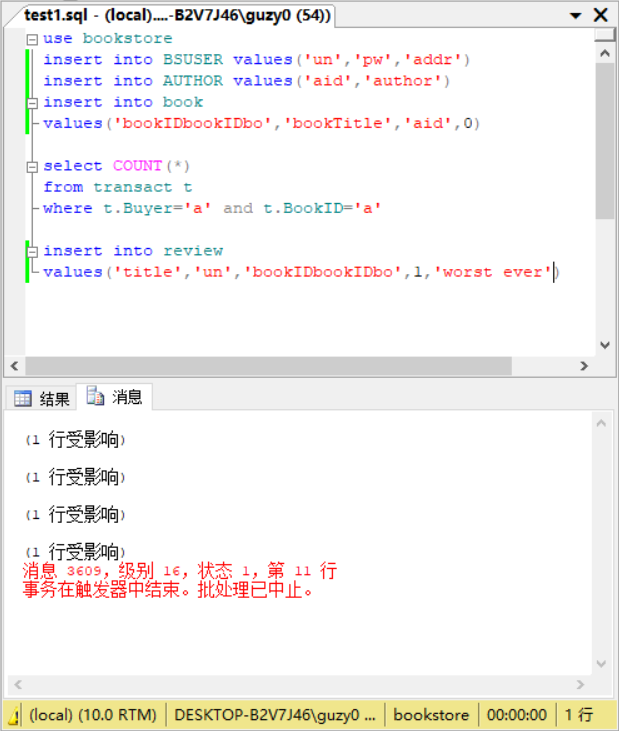
\includegraphics[width = 0.5 \textwidth]{test1me.png}}
\end{figure}
可以看出,用户'un'对书'bookIDbookIDbo'的交易为0,触发器致使'un'评论失败。
\subsubsection{交易}
购买书的时候,有以下几点:
\begin{enumerate}
    \item 书的数量要大于0。
    \item 买完后书的数量减1。
    \item 书单上标记已购此书。
\end{enumerate}
实现如下:
\begin{lstlisting}
create trigger t_transact on TRANSACT for insert as
if (select quantity from book, inserted where ISBN=inserted.BookID) <= 0
begin
rollback transaction
end
update book set quantity=quantity-1 where ISBN=(select BookID from inserted)
update bookmark_book set Owned=1 where BookID=(select BookID from inserted)
and Owner=(select Buyer from inserted)
\end{lstlisting}
测试如下:
\begin{figure}[H]
    \subfigure{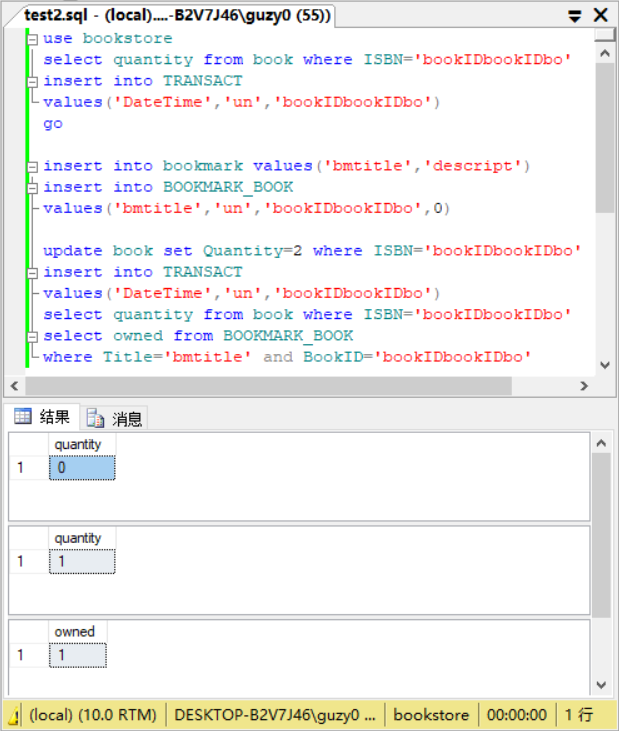
\includegraphics[width = 0.5 \textwidth]{test2re.png}}
    \subfigure{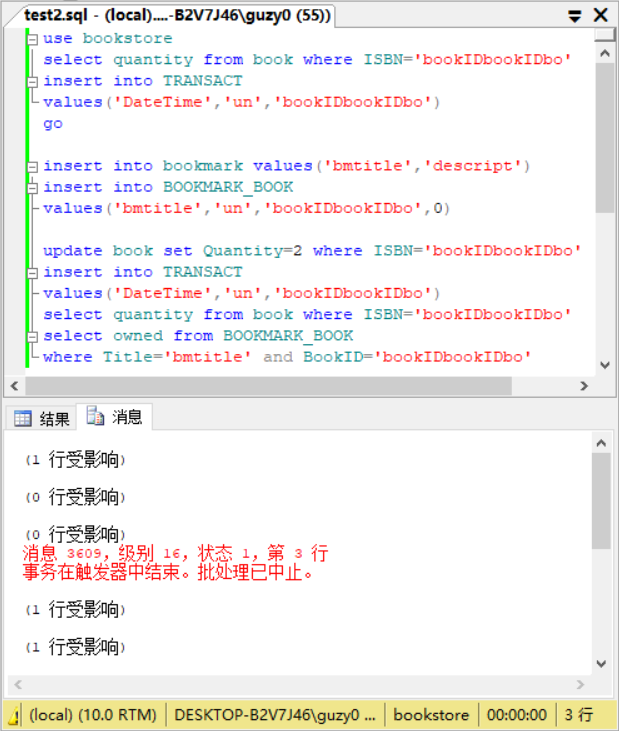
\includegraphics[width = 0.5 \textwidth]{test2me.png}}
\end{figure}
可以看出,书的数量是0,触发器致使'un'交易失败。设置此书于书单'bmtitle'中且标记为无此书,更新书的数量为2。之后再插入交易,发现成功,且交易后书的数量变为1,书单中标记为拥有此书。
\subsection{可能出现的不一致问题}
由于触发器并不是原子操作,在多用户多事务并发的环境下插入交易时可能出现不一致的情况。考虑此时某本书只有一个,事务A在刚刚判断完$quantity>0$而未修改quantity并提交,此时事务B也判断会
认为$quantity>0$,最终结果是一本书插入了两条交易。下面在触发器判断后和插入前加一个10秒延迟来模拟这种现象。test3.sql代码截图不全,因而在此放出:
\begin{lstlisting}
use bookstore
drop trigger t_transact
go
create trigger t_transact on TRANSACT for insert as
if (select quantity from book, inserted where ISBN=inserted.BookID) <= 0
begin
rollback transaction
end
waitfor delay '00:00:10'
update book set quantity=quantity-1 where ISBN=(select BookID from inserted)
update bookmark_book set Owned=1 where BookID=(select BookID from inserted)
and Owner=(select Buyer from inserted)
go

update book set quantity=1 where ISBN='bookIDbookIDbo'
begin tran
set transaction isolation level read committed
select quantity from book where ISBN='bookIDbookIDbo'
insert into TRANSACT
values('DateTime1','un','bookIDbookIDbo')
commit tran
\end{lstlisting}
其主要功能就是在t\_transact的判断语句和插入语句之间加一个延迟,将书quantity设为1并执行事务插入一条交易。运行结果如下:
\begin{figure}[H]
    \subfigure{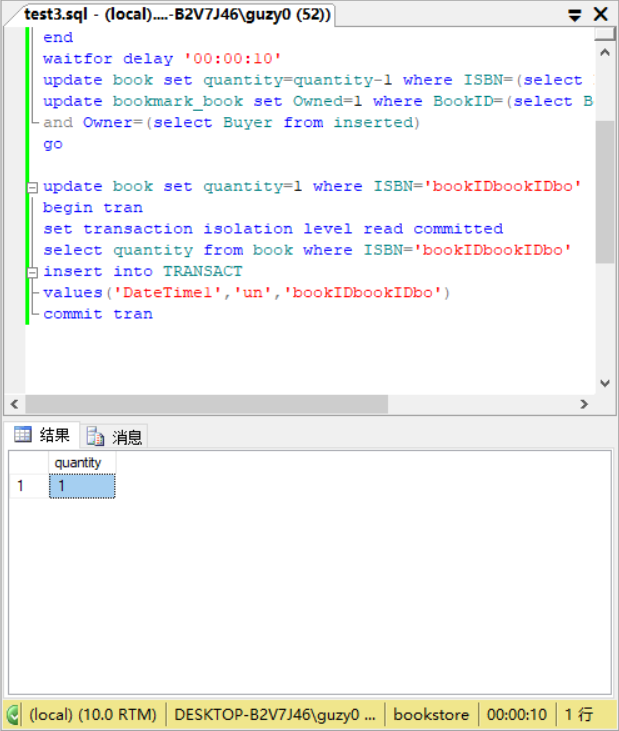
\includegraphics[width = 0.5 \textwidth]{test3re.png}}
    \subfigure{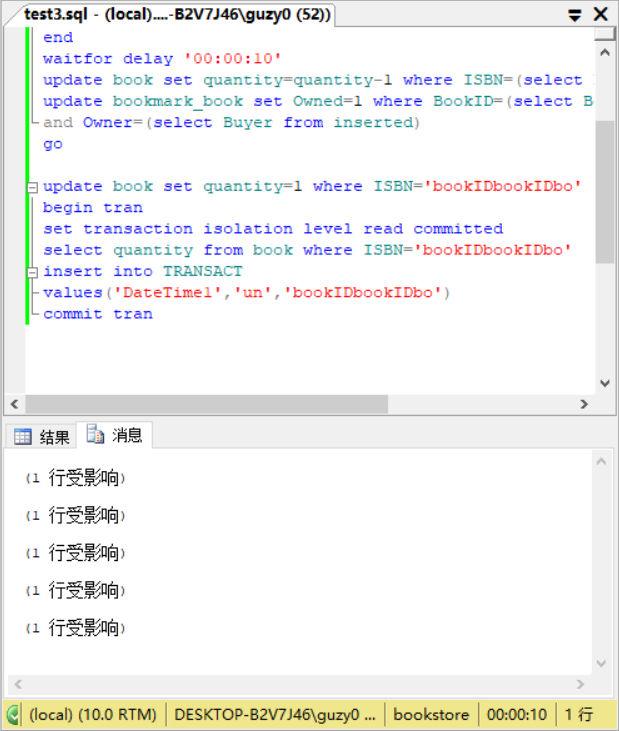
\includegraphics[width = 0.5 \textwidth]{test3me.png}}
\end{figure}
上面事务执行的同时,执行如下事务:
\begin{figure}[H]
    \subfigure{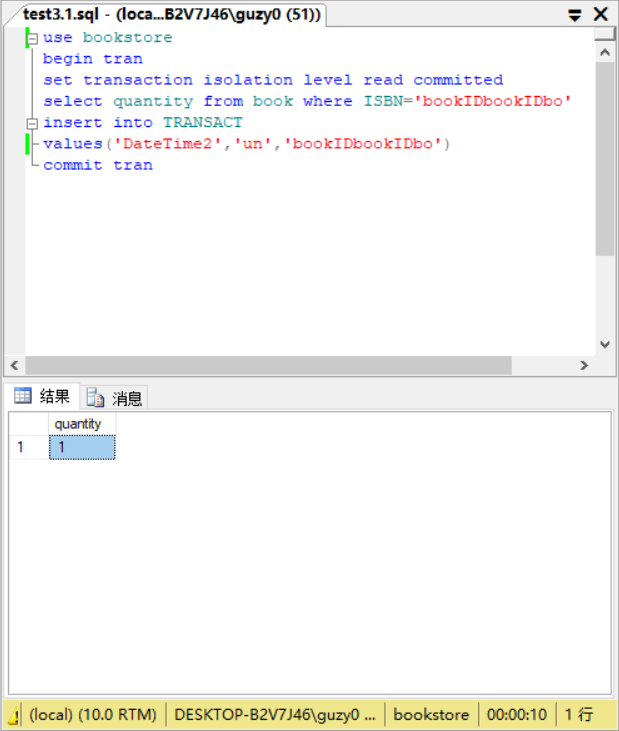
\includegraphics[width = 0.5 \textwidth]{test3.1re.png}}
    \subfigure{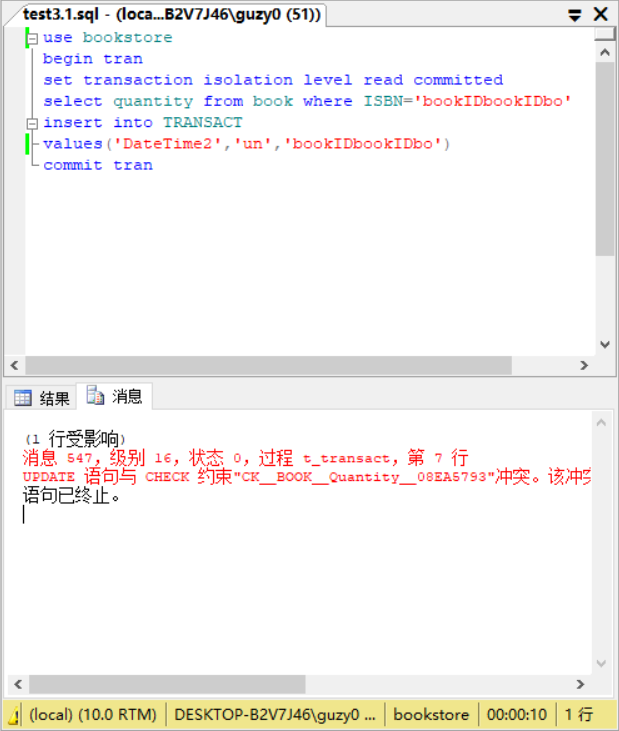
\includegraphics[width = 0.5 \textwidth]{test3.1me.png}}
\end{figure}
可以发现,两个事务都读到书的quantity为1,因此两个事务都没被回滚,执行了插入语句。但是由于quantity的约束要求大于等于0,其中一个事务的trigger更新会失败,导致trigger失败进而导致
插入语句失败。因此update语句和对quantity的约束已经防止了此类不一致的发生,因而提前判断quantity也是没必要的,因而改成:
\begin{lstlisting}
create trigger t_transact on TRANSACT for insert as
update book set quantity=quantity-1 where ISBN=(select BookID from inserted)
update bookmark_book set Owned=1 where BookID=(select BookID from inserted)
and Owner=(select Buyer from inserted)
\end{lstlisting}
%\clearpage
%\bibliography{E:/Papers/LiuLab}
%\bibliographystyle{apalike}
\end{document}
%%% Local Variables:
%%% mode: latex
%%% TeX-master: t
%%% End:
